\section{Introduction}
\label{sec:introduction}

Docking provides an underwater vehicle a place to recharge, offload its data and perform long-running tasks without surfacing or returning to a support ship. Since surfacing and recovery are slow, and weather-limited and expensive, removing them from the mission cycle is what makes long deployments and resident vehicle systems possible. The engineering challenge concentrates in the last few metres of the dock approach (Figure~\ref{fig:docking-problem}), in which if this stage goes wrong, the vehicle may collide with the dock, or abort and spend unnecessary time and energy retrying.

\begin{figure}[H]
    \centering
    % Annotated docking-problem figure for the Introduction.
% Image: Gazebo screenshot, BlueROV2 seen from behind on approach with the
% marker-equipped dock ahead. Coordinates are normalised to the image
% (0,0 = bottom left).
\begin{tikzpicture}
  \node[anchor=south west, inner sep=0] (img) {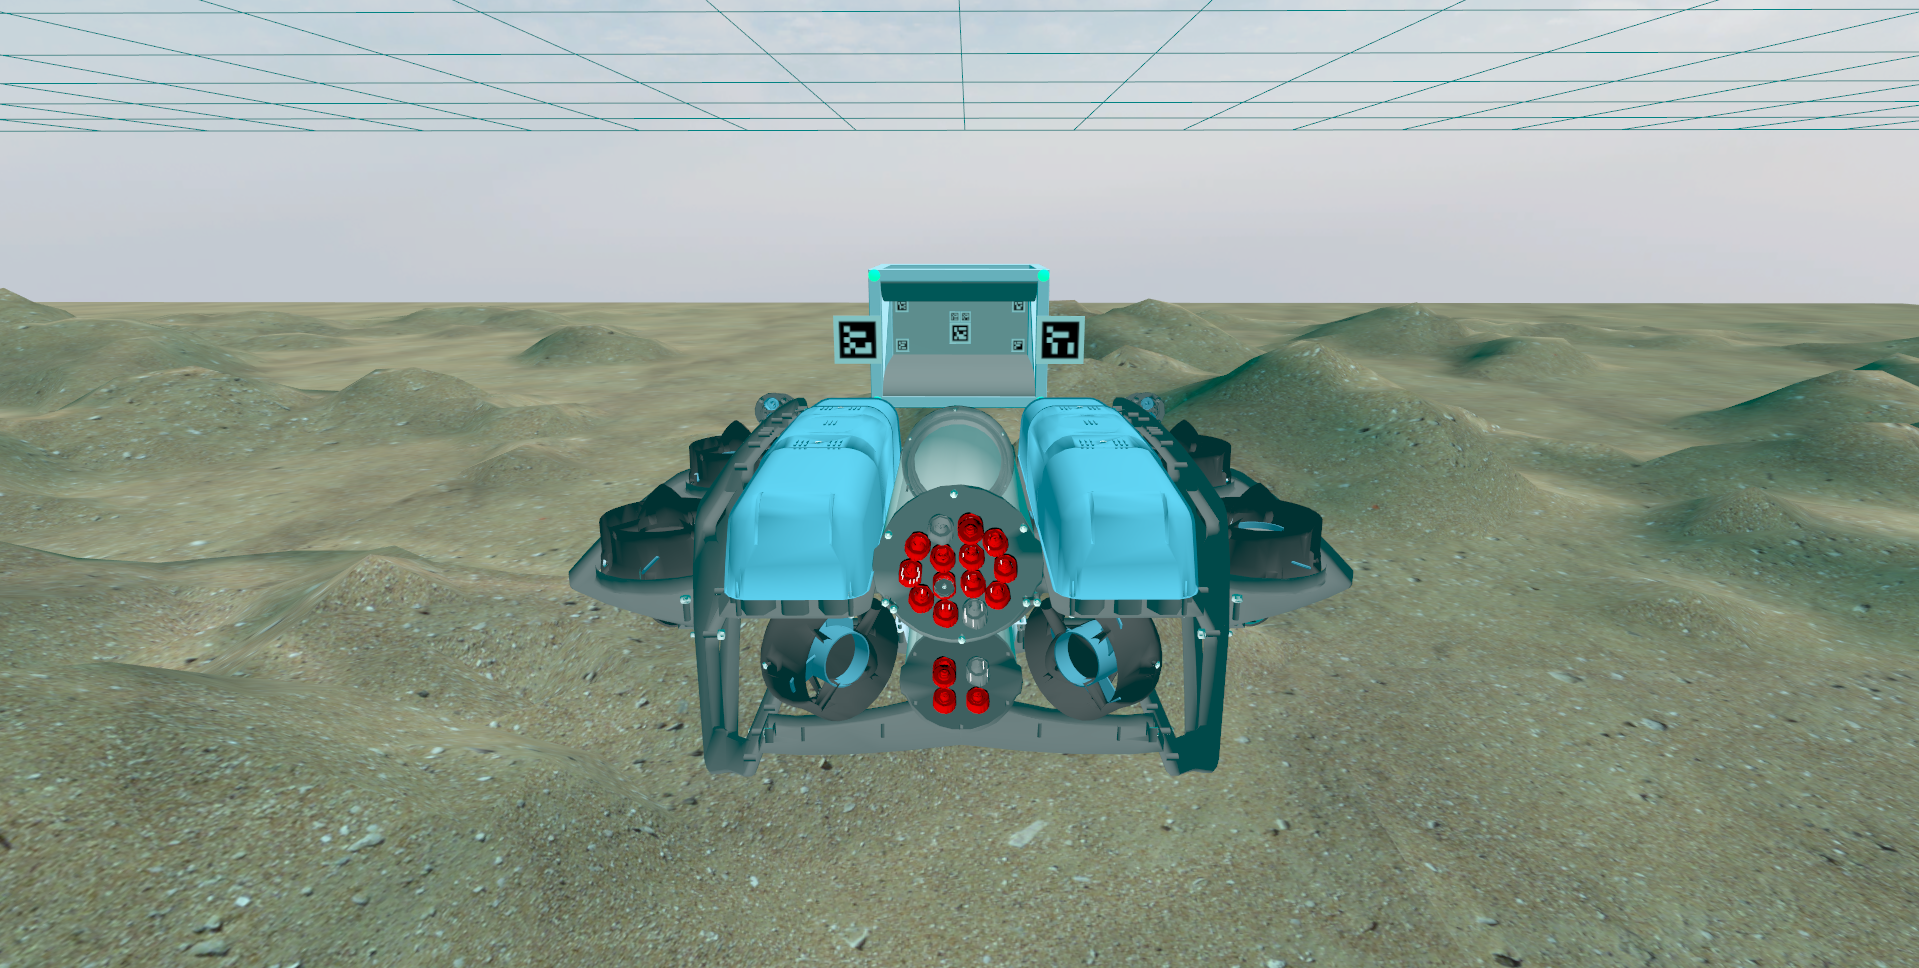
\includegraphics[width=0.85\textwidth]{Images/docking_problem.png}};
  \begin{scope}[x={(img.south east)}, y={(img.north west)},
    lab/.style={font=\scriptsize\bfseries, text=white, align=center, fill=black, fill opacity=0.55,
        text opacity=1, inner sep=3pt, rounded corners=1pt},
    arr/.style={orange, thick, -{Stealth[length=1.6mm]}}]
    \draw[white, thin, dashed, opacity=0.8] (0.50,0.56) -- (0.435,0.635);
    \draw[white, thin, dashed, opacity=0.8] (0.50,0.56) -- (0.565,0.635);
    \node[lab] (lrov) at (0.16,0.55) {BlueROV2\\forward camera};
    \draw[arr] (lrov.east) to[bend right=10] (0.36,0.44);
    \node[lab] (ldock) at (0.83,0.82) {docking station\\passive ArUco markers};
    \draw[arr] (ldock.south) to[bend left=10] (0.575,0.70);
    \node[lab] (lsway) at (0.24,0.82) {wave-driven sway};
    \draw[arr, <->] (0.41,0.77) -- (0.57,0.77);
  \end{scope}
\end{tikzpicture}

    \caption{The terminal docking problem: the vehicle must fly the final
        metres onto a docking station using its forward camera and marker detection, while the dock itself sways with the sea above.}
    \label{fig:docking-problem}
\end{figure}

Conventionally, a docking mission is staged by sensing modality, like acoustic or electromagnetic homing, to bring the vehicle from long range into the vicinity of the dock, then vision takes over for the final metres, where the precision requirement is tightest. This thesis addresses only the vision stage; homing and the mechanical capture are out of scope. Within the vision stage, two practical difficulties receive little attention in the literature. First, a real dock is rarely still, since moored and suspended structures inherit the wave motion of the sea around them. Second, the water limits how far a camera can see the dock at all, so marker visibility itself becomes a design constraint.

The work is split into two parts (Figure~\ref{fig:workflow}). Part~A develops the complete docking pipeline in simulation (marker fusion, a Kalman filter for the dock pose, and phase control) and runs it against a dock swaying at certain wave periods.\footnote{The docking stack and simulation fork are available at \url{https://github.com/alanchoi00/bluerov2-docking} and \url{https://github.com/alanchoi00/blue-sim}.} A docking trial sweep through the sway periods is performed to determine where the docking breaks down and the failure analysis explains why. Part~B takes the marker detector into real water where a pool capture measures detection against marker size, maximum detection range and the water's attenuation coefficient, and the same frames are then processed with artificial turbidity to produce a marker sizing rule. This split is necessary since the Gazebo simulator is able to exercise the closed loop, but cannot render water optics; the pool test captures have real optics but no control loop.

\begin{figure}[H]
    \centering
    \begin{tikzpicture}[font=\scriptsize, >={Stealth[length=2mm]},
  blk/.style={draw, rounded corners=2pt, align=center, inner sep=3pt, minimum height=6.5mm, minimum width=34mm},
  sumbox/.style={draw, rounded corners=2pt, align=center, inner sep=3pt, minimum height=6.5mm, minimum width=34mm, fill=black!6},
  lbl/.style={font=\scriptsize\bfseries, anchor=west}]

  % Part A column (closed-loop simulation)
  \node[blk] (a1) {swaying dock\\ \tiny Gazebo, wave-band periods};
  \node[blk, below=4.5mm of a1] (a2) {onboard camera};
  \node[blk, below=4.5mm of a2] (a3) {perception\\ \tiny marker fusion + Kalman filter};
  \node[blk, below=4.5mm of a3] (a4) {guidance and control\\ \tiny PBVS, coarse-to-fine state machine};
  \node[blk, below=4.5mm of a4] (a5) {vehicle motion};
  \draw[->] (a1) -- (a2);
  \draw[->] (a2) -- (a3);
  \draw[->] (a3) -- (a4);
  \draw[->] (a4) -- (a5);
  \draw[->] (a5.west) to[bend left=40] node[left, align=center]{\tiny moving\\ \tiny camera} (a2.west);

  % Part B column (real-water sensing, open loop)
  \node[blk, right=24mm of a1] (b1) {marker board in pool water\\ \tiny hand-held walk-backs};
  \node[blk, below=4.5mm of b1] (b2) {ArUco detection\\ \tiny scored per marker and frame};
  \node[blk, below=4.5mm of b2] (b3) {envelope measurements\\ \tiny detection vs apparent size, max\\ \tiny range, attenuation coefficient};
  \node[blk, below=4.5mm of b3] (b4) {synthetic turbidity stress\\ \tiny re-attenuate the same frames};
  \draw[->] (b1) -- (b2);
  \draw[->] (b2) -- (b3);
  \draw[->] (b3) -- (b4);

  % group boxes
  \node[draw, dashed, rounded corners=3pt, inner sep=3mm, fit=(a1)(a5)] (boxA) {};
  \node[draw, dashed, rounded corners=3pt, inner sep=3mm, fit=(b1)(b4)] (boxB) {};
  \node[lbl, anchor=south west] at (boxA.north west) {A: docking dynamics (sim)};
  \node[lbl, anchor=south west] at (boxB.north west) {B: sensing envelope (real water)};

  % synthesis
  \node[sumbox, below=8mm of $(boxA.south)!0.5!(boxB.south)$, minimum width=62mm]
  (syn) {operating envelope and dock design rules\\ \tiny sway-period limit, capture-interface numbers, pixel budget, marker sizing};
  \draw[->] (boxA.south) -- (syn.north -| boxA.south);
  \draw[->] (boxB.south) -- (syn.north -| boxB.south);
\end{tikzpicture}

    \caption{How the two parts fit together. The return arrow in Part~A is
        the closed control loop; Part~B is an open-loop measurement chain;
        their outputs combine into the envelope and design rules.}
    \label{fig:workflow}
\end{figure}

The objective of this thesis is to build and validate a terminal docking stage from passive markers and computer vision, the approach available to a low-cost ROV, and to establish its operating envelope. In simulation, the system docks autonomously onto a swaying dock, cleanly down to 8~s sway periods at 0.1~m amplitude. The swept periods are mapped to the NSW sea states to determine suitable dock depths. The sweep also uncovered a control instability: estimating the dock's velocity through a moving camera lets the vehicle's own motion corrupt the estimate, and at short sway periods this feedback destabilises the approach, while a simpler design that never estimates dock velocity is unaffected. On the sensing side, measurements on real underwater imagery established the perception envelope: a marker needs around 27 pixels of apparent size to be detected, maximum detection range is about 35 times the marker side, the water's attenuation coefficient was measured from the imagery itself, and inverting these numbers yields a sizing rule for the dock's markers.

Section~\ref{sec:literature-review} reviews the docking literature and states the research gap. Section~\ref{sec:methodology} describes the system and the experimental method for both parts. Section~\ref{sec:results} presents and discusses the results, and Section~\ref{sec:conclusion} concludes with future work.
